For the Alloy part we focused on the interview state machine, specially in the slot assignment process. The purpose of this choice was to ensure that the scheduling mechanism is consistent and to further explain its details.

First, we started with some signature definitions that helped us to properly define our model:

\lstinputlisting[language=alloy]{Files/alloy-code/signature-defs.tex}


Then, we moved on to some predicates to help us model and understand possible user actions that will trigger state transitions.

\lstinputlisting[language=alloy]{Files/alloy-code/predicates.tex}

Lastly, we wrote some facts to ensure the proper behavior of our model:

\lstinputlisting[language=alloy]{Files/alloy-code/facts.tex}

\subsection{Examples}

\begin{figure}[h]
\centering
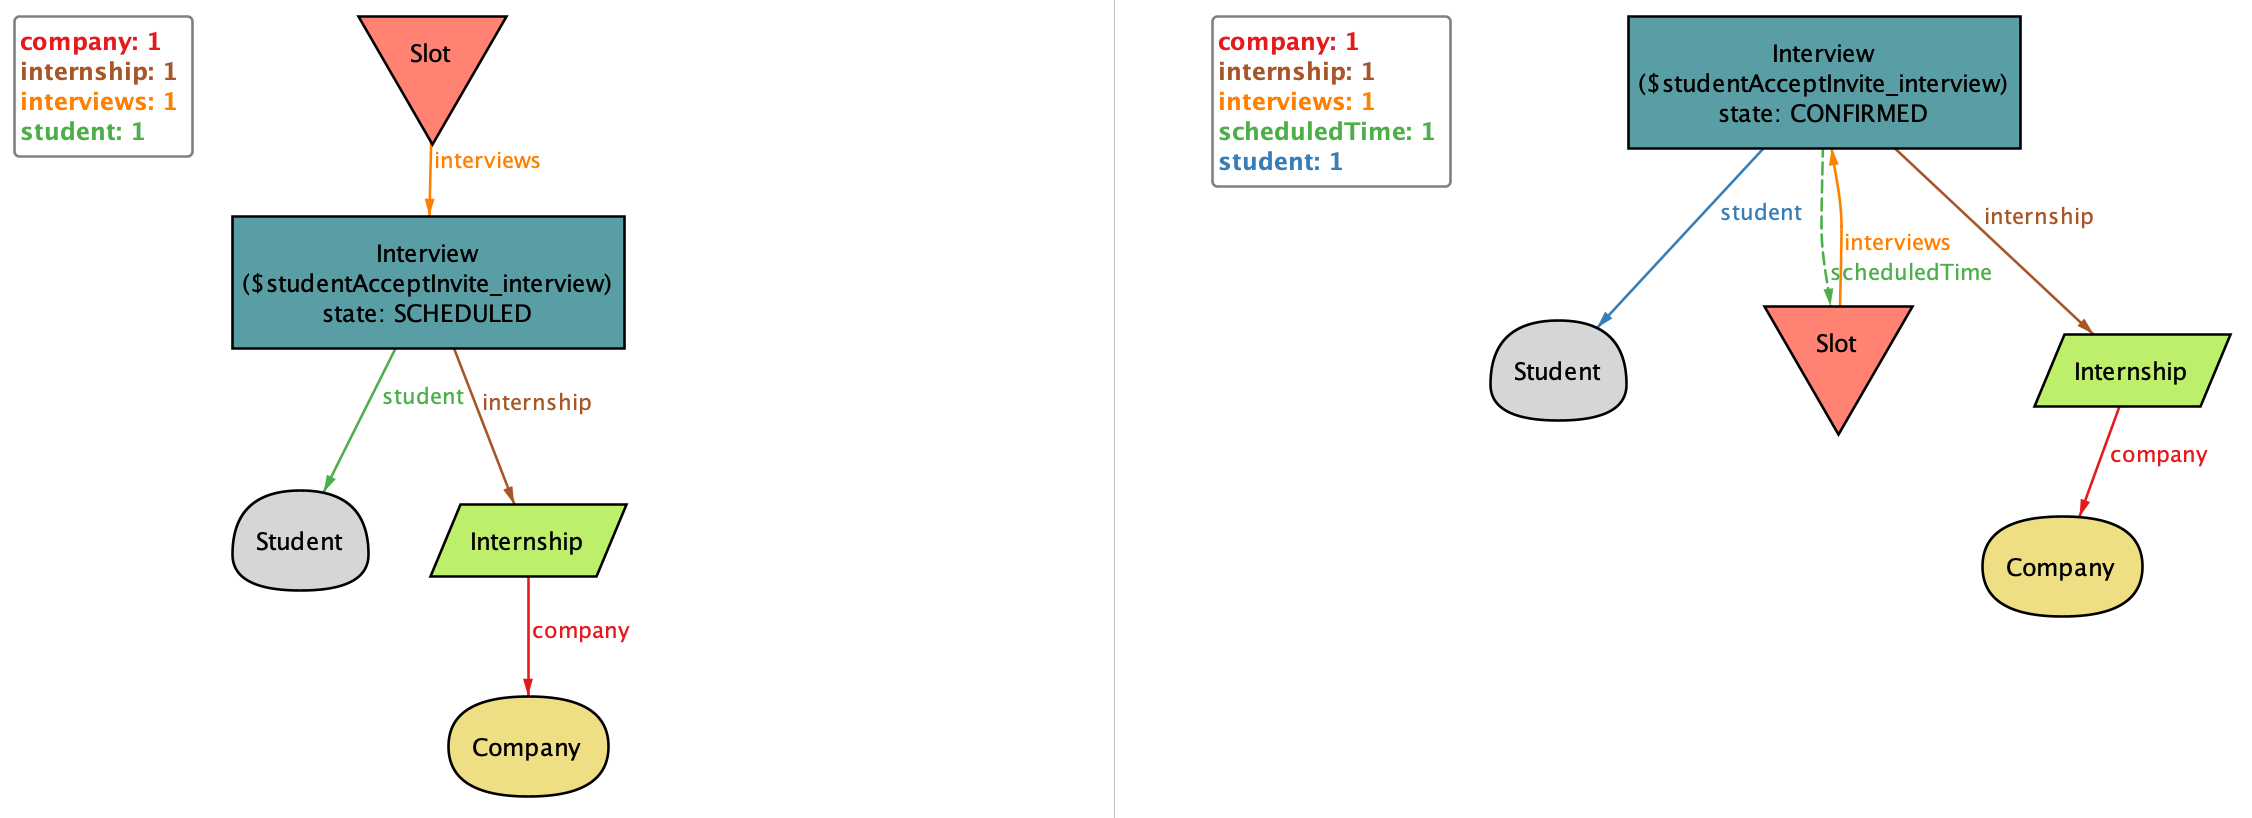
\includegraphics[width=\textwidth]{Images/caseOneInterview-1.png}
\caption{\label{fig:alloy-example-1-1} Example 1: One interview, steps 1 and 2}
\end{figure}

\begin{figure}[h]
\centering
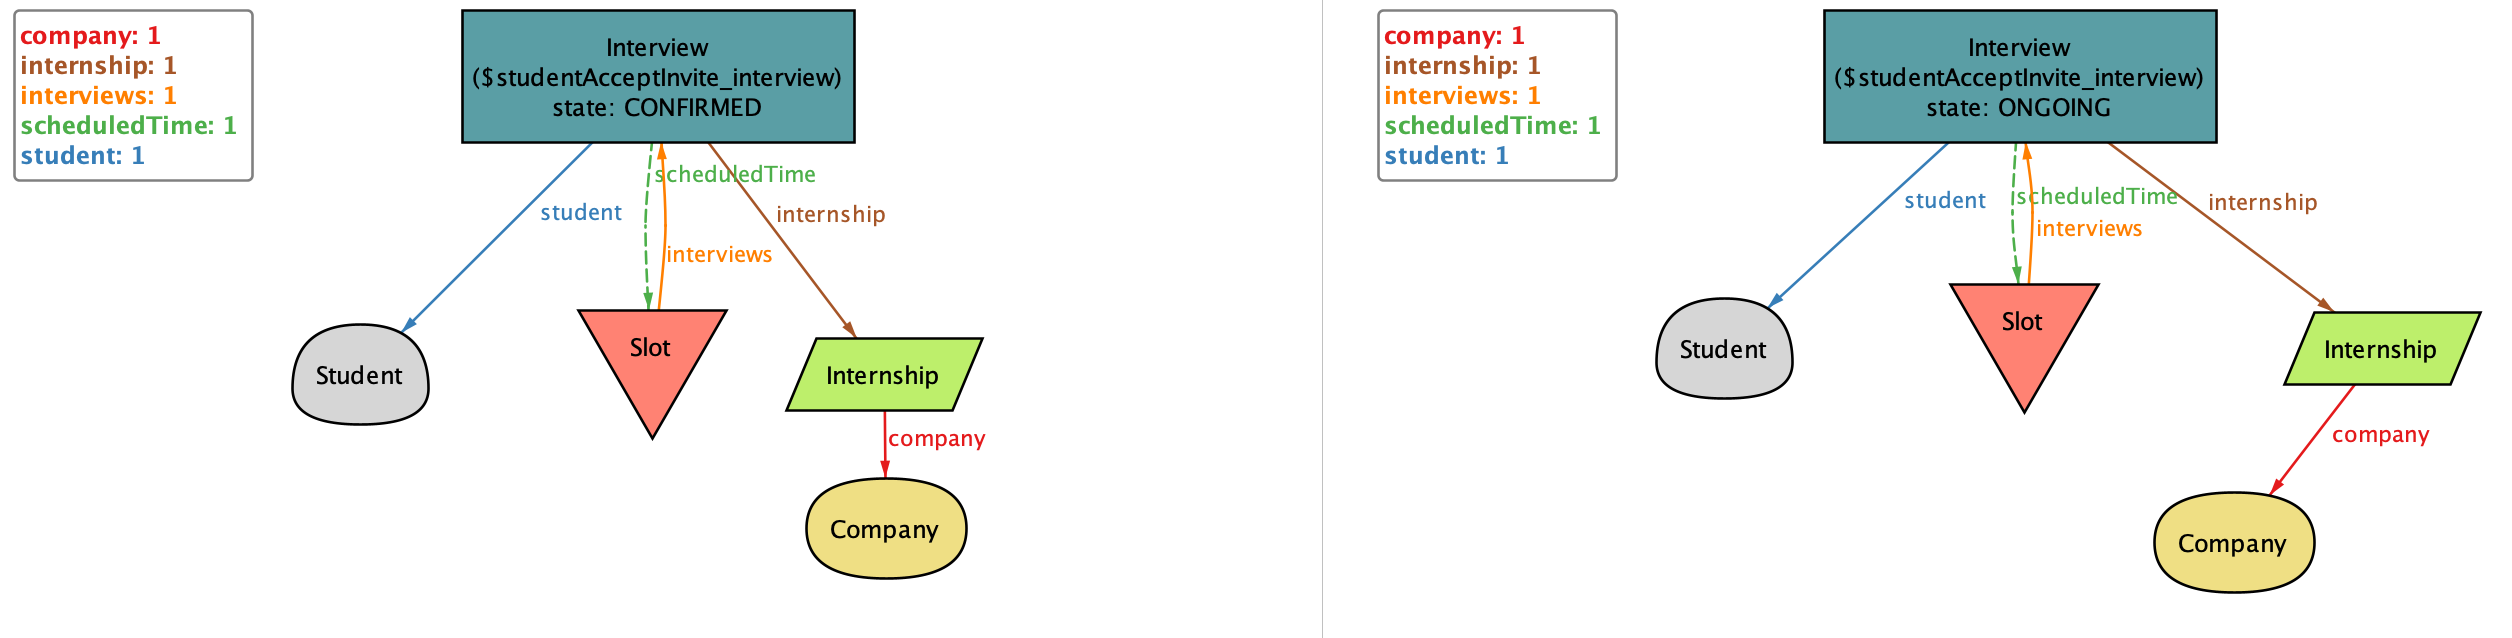
\includegraphics[width=\textwidth]{Images/caseOneInterview-2.png}
\caption{\label{fig:alloy-example-1-2} Example 1: One interview, steps 3 and 4}
\end{figure}

\begin{figure}[h]
\centering
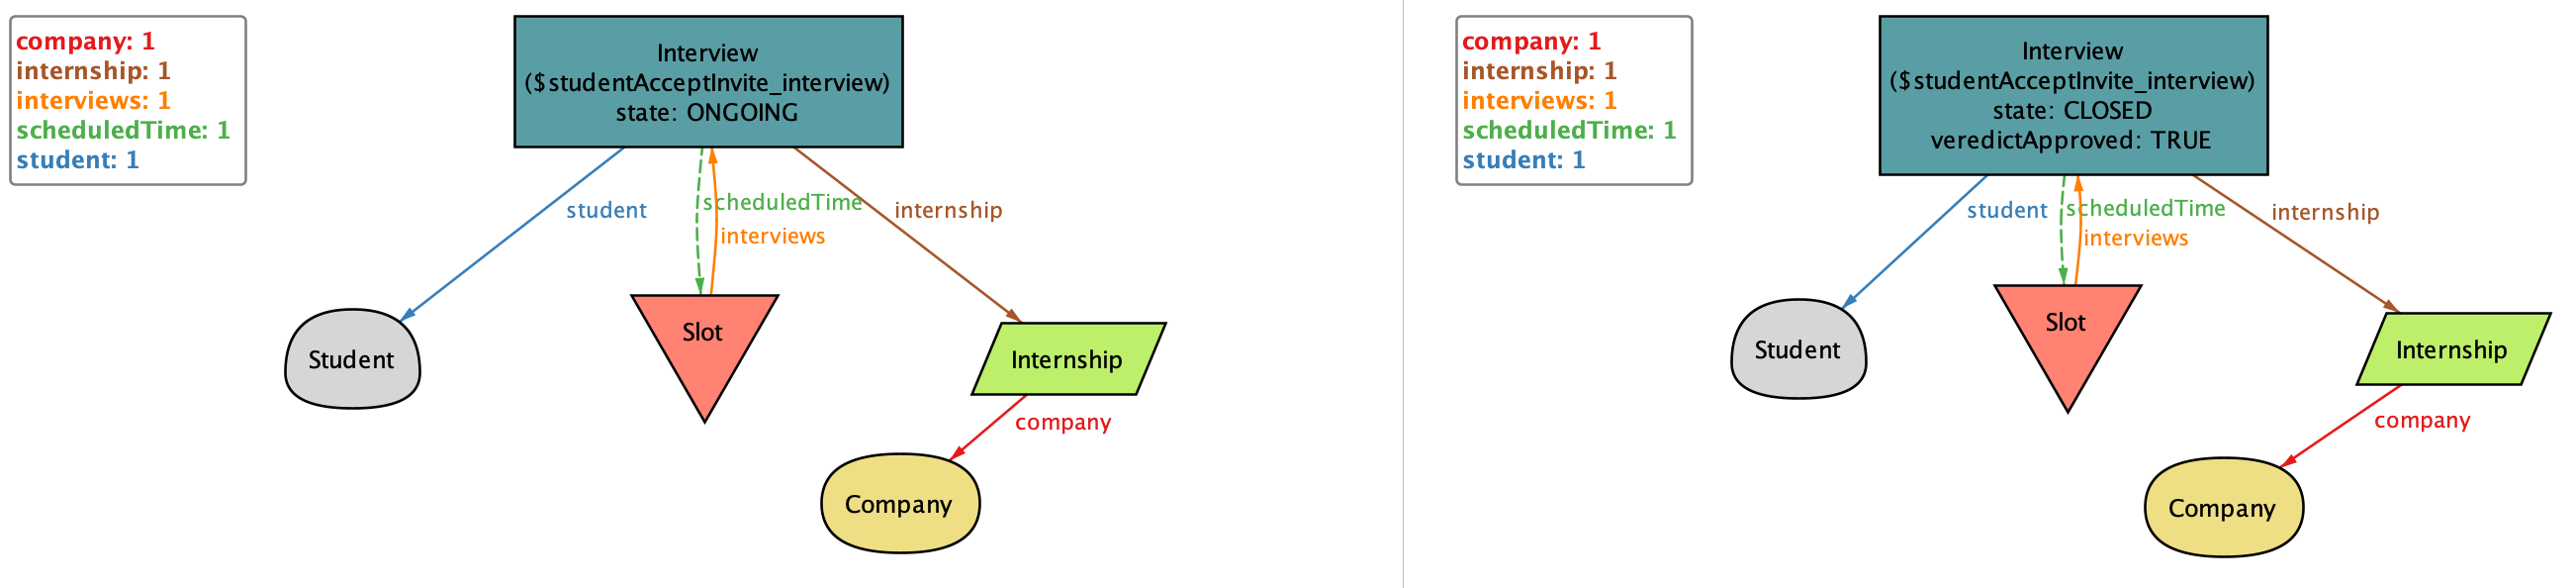
\includegraphics[width=\textwidth]{Images/caseOneInterview-3.png}
\caption{\label{fig:alloy-example-1-3} Example 1: One interview, steps 5 and 6}
\end{figure}

\begin{figure}[h]
\centering
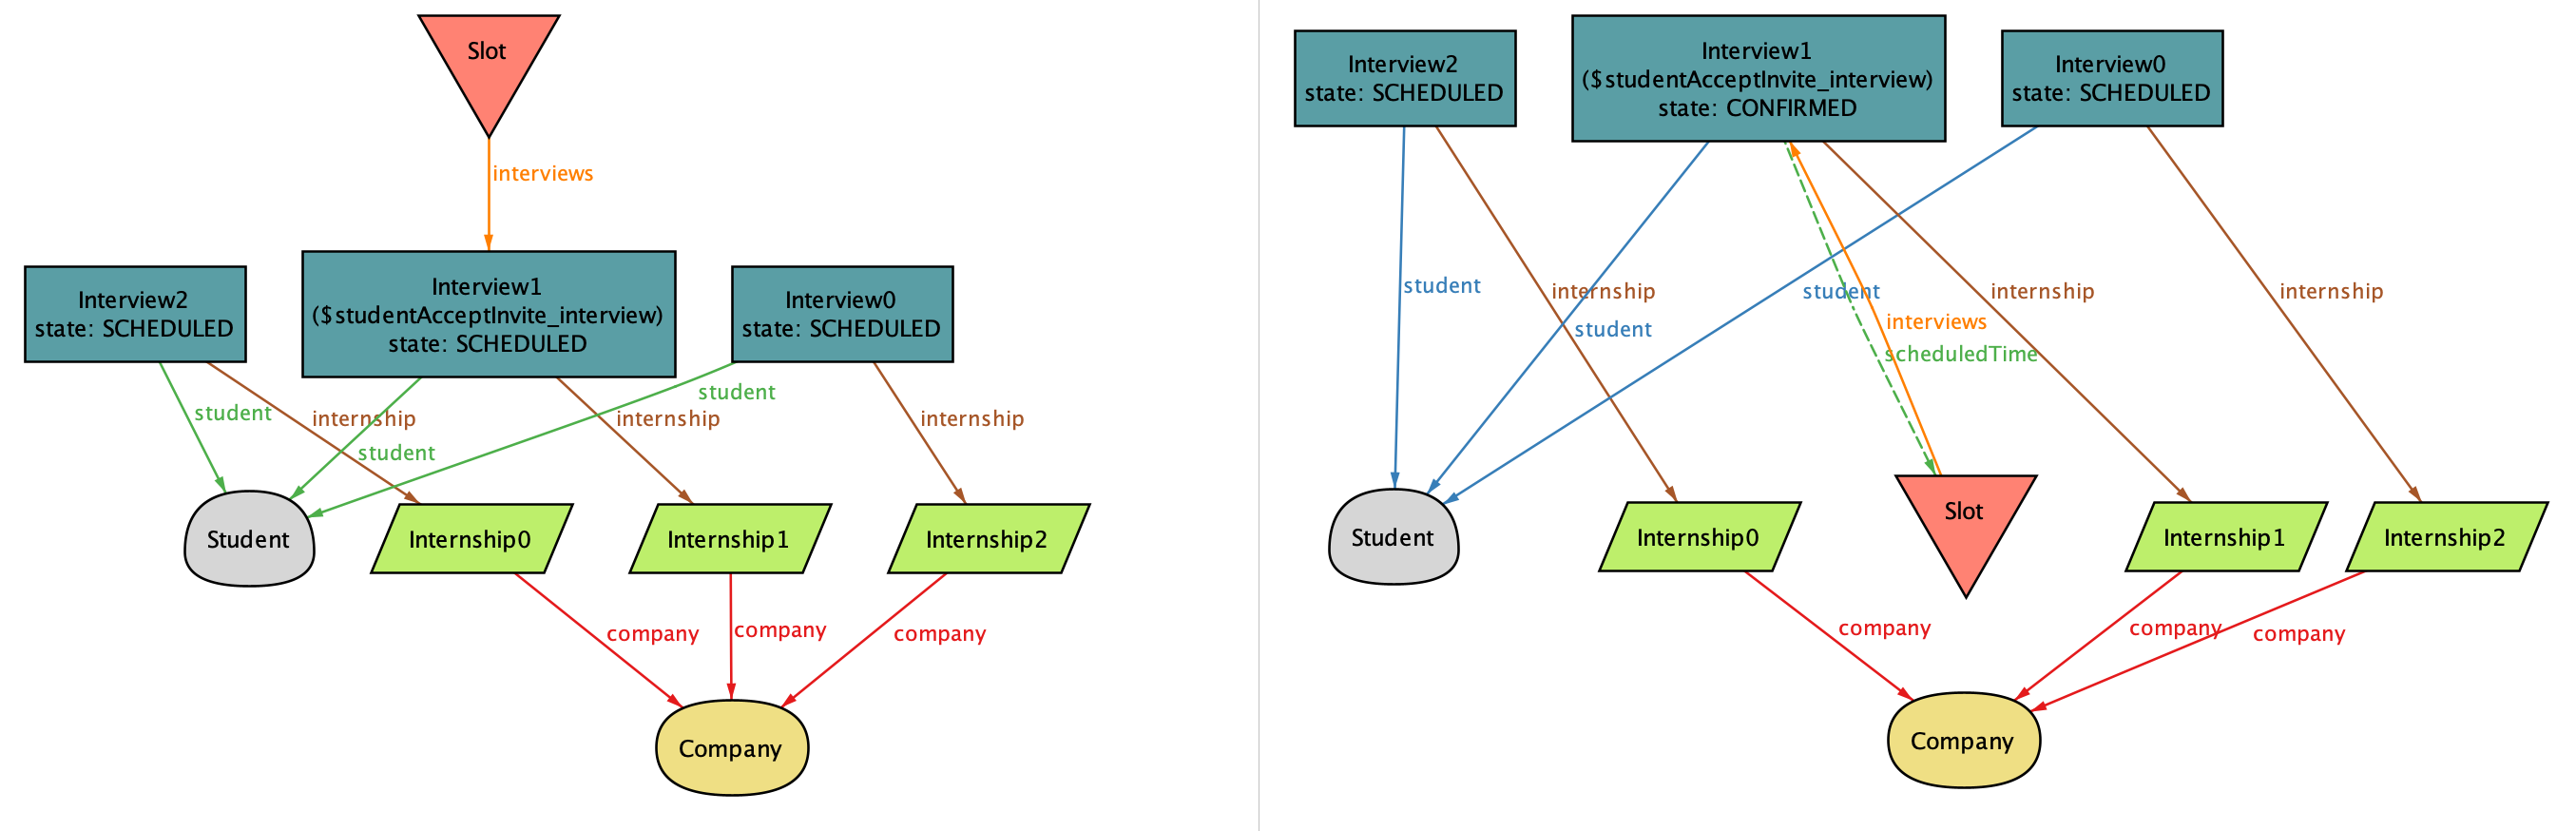
\includegraphics[width=\textwidth]{Images/caseThreeInterviews-1.png}
\caption{\label{fig:alloy-example-2-1} Example 2: Three interviews, steps 1 and 2}
\end{figure}

\begin{figure}[h]
\centering
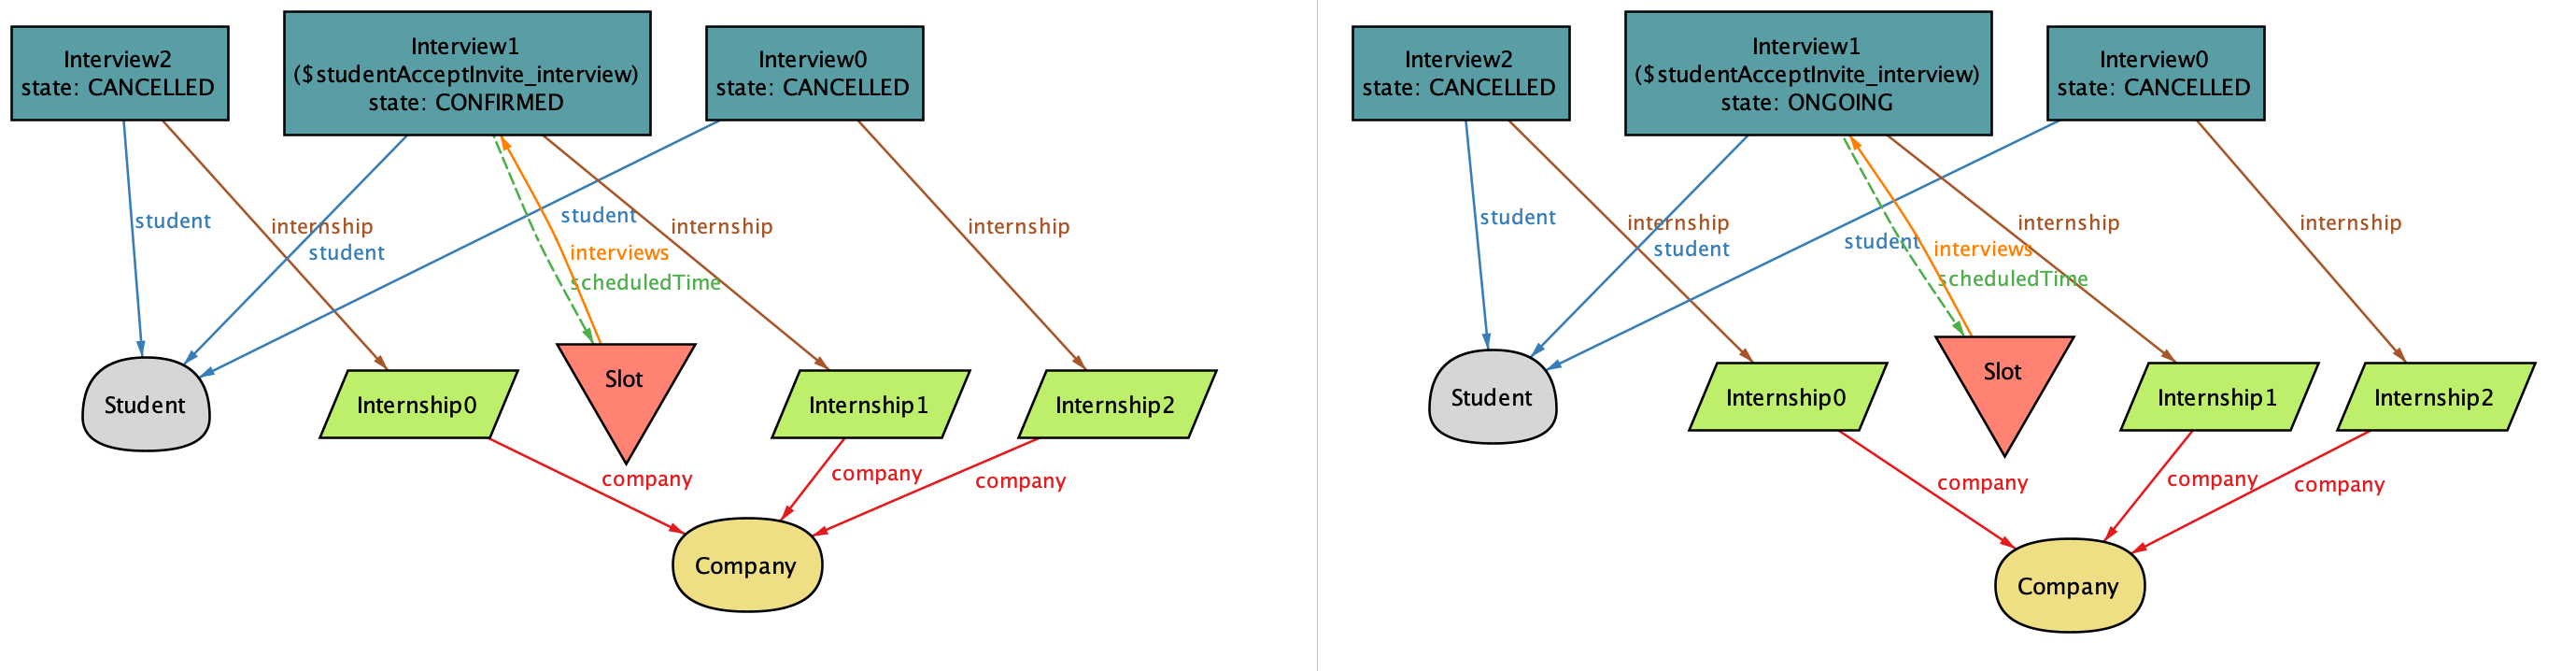
\includegraphics[width=\textwidth]{Images/caseThreeInterviews-2.png}
\caption{\label{fig:alloy-example-2-2} Example 2: Three interviews, steps 3 and 4}
\end{figure}

\begin{figure}[h]
\centering
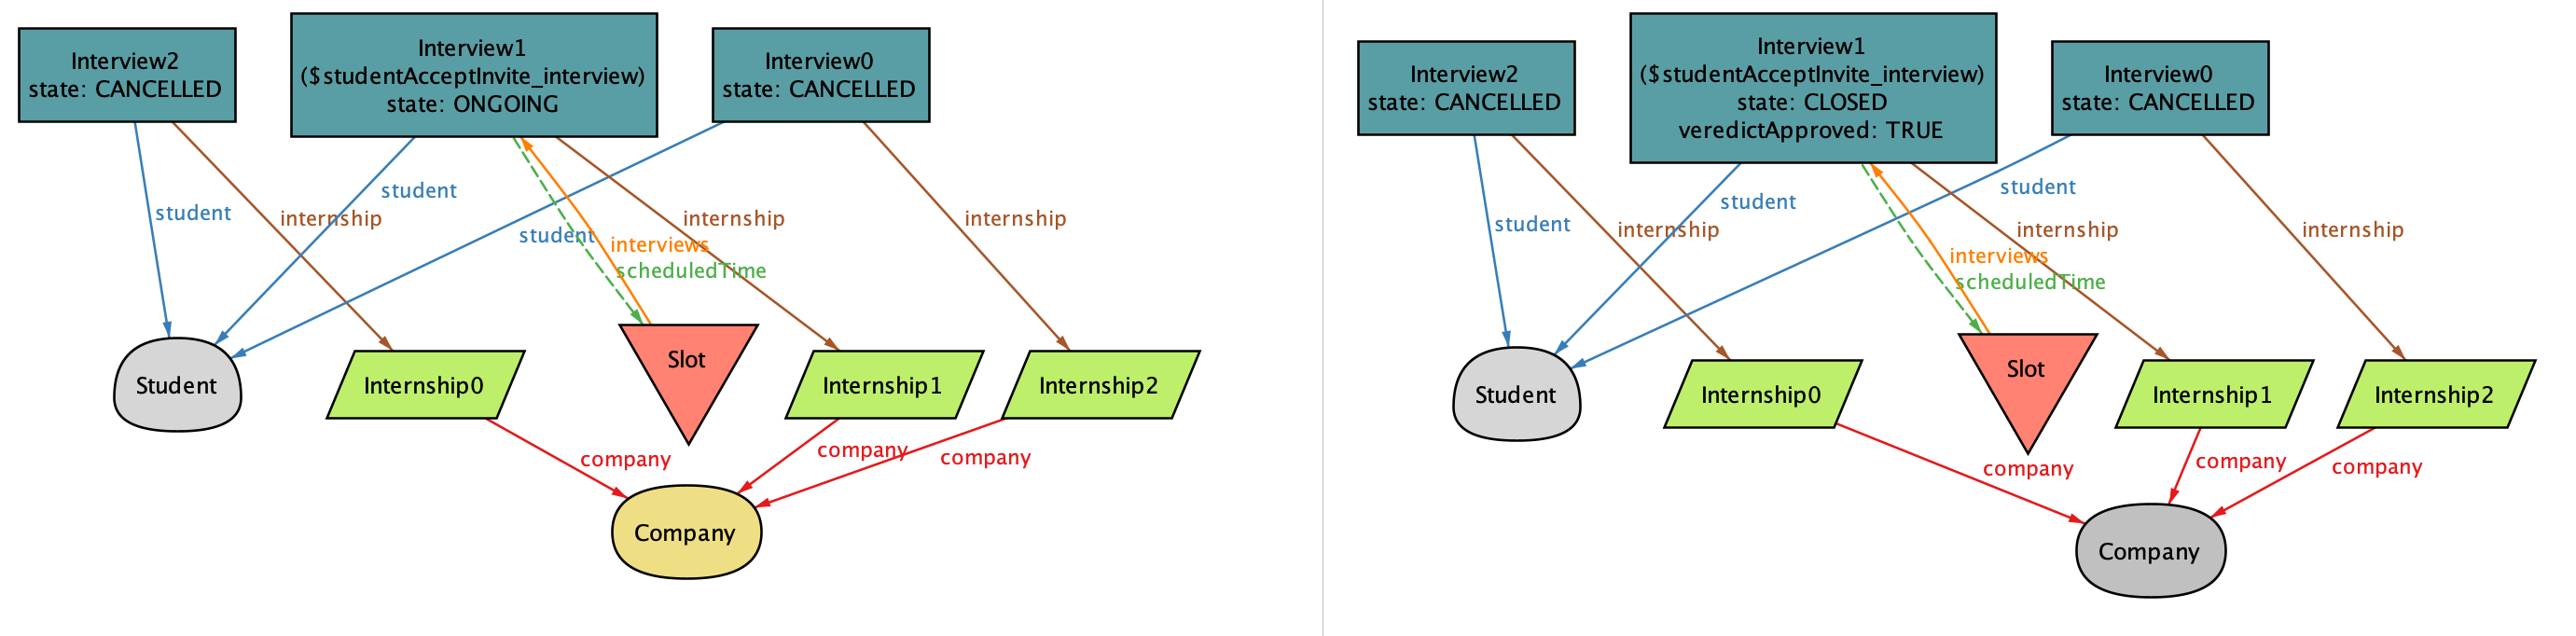
\includegraphics[width=\textwidth]{Images/caseThreeInterviews-3.png}
\caption{\label{fig:alloy-example-2-3} Example 2: Three interviews, steps 5 and 6}
\end{figure}